%!TEX root = ../../sbc-template.tex

\emph{Deep Learning} (DL), também conhecido como Aprendizagem Profunda, compreende um conjunto de técnicas de ML que podem ser aplicadas em problemas de aprendizado supervisionado e não-supervisionado. A principal característica dos modelos neste domínio é a capacidade de representar e reconhecer características sucessivamente complexas, por meio da adição de níveis ou camadas de operações não-lineares em sua arquiteturas, a exemplo das nas redes neurais profundas, máquinas de Boltzmann profundas e fórmulas proposicionais. Modelos deste tipo ganharam popularidade ao se mostraram capazes de resolver problemas complexos com um desempenho cada vez maior \cite{bengio2009learning}.

% Desnecessário
%Há dois aspectos recorrentes nas diversas descrições de DL presentes atualmente: ($1$) modelos que consistem de camadas ou estágios sucessivos de processamento de informações não-lineares; e ($2$) métodos para aprendizado supervisionado ou não-supervisionado de representação de características em camadas sucessivamente mais altas ou abstratas.

A melhoria do desempenho de modelos de DL é decorrente do aumento recente da quantidade de dados disponíveis sobre temas complexos, aliado ao aumento da disponibilidade de recursos computacionais para executar modelos mais robustos \cite{goodfellow2016deep,deng2014deep}. Alguns dados fornecidos pela IBM reforçam esta afirmação: em $2017$ foram gerados $2,5$ quintilhões de bytes de dados por dia, e $90\%$ do volume total de dados gerados até $2017$ no mundo foi criado somente nos últimos dois anos \cite{ibm2017bigdata}.

Para exemplificar o efeito da adição de camadas aos modelos de DL, a Figura \ref{fig:compara_redes} mostra uma visão geral do aumento da profundidade das camadas nas redes neurais profundas e o desempenho destas em problemas de detecção de objetos em imagens. Nota-se que, à medida que a profundidade aumenta, há uma diminuição no erro. Mais recentemente, isto também têm implicado na redução do número de parâmetros treináveis.  Este panorama reforça a hipótese de que a profundidade das camadas impacta positivamente na captura de características e que estes avanços têm tornado as tarefas mais factíveis, com uma diminuição do esforço computacional associado  \todo{Citação aqui é essencial. Pode ser a mesma da origem da figura}.


\begin{figure}[ht]
	\centering
	\caption{Evolução de profunidade, taxa de erro e número de parâmetros das redes neurais profundas com o passar dos anos. Fonte: \cite{mediumcnn}.}
	\label{fig:compara_redes}
	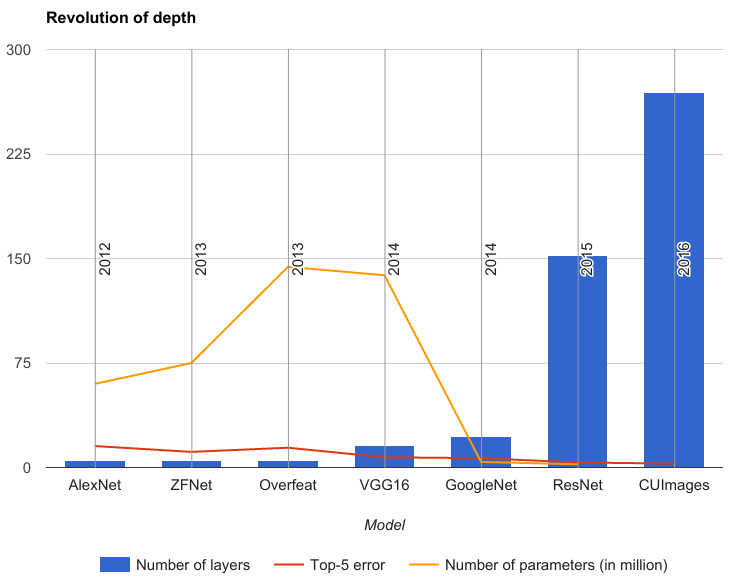
\includegraphics[width=0.8\textwidth]{img/compara_redes.png}
\end{figure}

\subsubsection{Breve Histórico}

O termo \emph{Deep Learning} não é recente, foi utilizado pela primeira vez por Dechter, no contexto da descoberta de todas as configurações de conflitos mínimas a fim de resolver um problema de satisfação de restrições
\cite{dechter1986learning}. Porém, ganhou força a partir de pesquisas sobre RNAs \emph{feedforward} com muitas camadas ocultas, também conhecidas por redes neurais profundas \cite{deng2014deep}.

% incompleto e inconsistente
%. Em ANO, foi utilizado para designar métodos que têm a ver com o DL moderno em PUBLICAÇÃO, que trata de TEMA. A partir daí, o termo passou a designar modelos compostos de várias camadas sucessivas de operações não lineares utilizados para o aprendizado de determinada tarefa.

Considera-se que o desenvolvimento de DL pode ser entendido em três partes. Na primeira, houve a proposição de modelos lineares simples, compostos apenas por um neurônio, a exemplo dos neurônios de McCulloch e Pitts \cite{mcculloch1943logical} e \emph{Perceptron} de Rosenblatt  \cite{rosenblatt1958perceptron}. A segunda parte, iniciada nos anos 1980, teve como eixo central a interconexão entre vários neurônios e a proposição do algoritmo \emph{back-propagation} para ajuste de pesos no treinamento das RNAs  \cite{rumelhart1986parallel,rumelhart1986backpropagation}. Com estas contribuições, houve muita aplicação das RNAs em diversos domínios. Ainda no final deste segundo momento, duas contribuições relevantes foram feitas: os modelos \emph{Long Short-Term Memory} (LSTM) e LeNet \cite{lenet}.   \todo[inline]{Complementar com importância da LeNet.}

A terceira fase têm um marco inicial mais definido: compreende o ano de $2006$ e a publicação de um artigo por Hinton et al. apresentando as \emph{deep belief networks} \cite{hinton2006fast}. Neste tipo de RNA, o aprendizado é realizado de forma não-supervisionada e as camadas que compõem a rede atuam como reconhecedoras de características. A partir deste momento, a utilização de DL se popularizou.

Na conjectura atual, modelos de DL têm superado significativamente o estado da arte de modelos inteligentes em diversas competições em todo o mundo. A \emph{ImageNet Large Scale Visual Recognition Challenge} (ILSVRC) é uma competição em que equipes de pesquisa avaliam seus algoritmos em um conjunto de dados fornecido, e competem para chegar à melhor acurácia em várias tarefas de reconhecimento visual automático. Em 2011, os melhores resultados de  classificação no ILSVRC tinham por volta de $25\%$ de erro nas tarefas propostas. Em 2012, o modelo AlexNet, uma rede neural convolucional proposta segundo as ideias de DL, atingiu apenas $16,4\%$ de erro, propondo um ganho dificilmente visto entre duas edições sucessivas da competição.

O gráfico da Figura \ref{fig:compara_redes} sintetiza o histórico da competição ILSVRC, em que a partir do ano de 2012 houve a introdução de modelos baseados em DL. O histograma mostra a diminuição do erro na tarefa de aprendizado proposta e a linha laranja enfatiza o número de camadas ocultas utilizadas nos modelos vencedores.

\begin{figure}[ht]
	\centering
	\caption{Evolução do erro dos modelos vencedores da competição ILSVRC pela profundidade das redes neurais \cite{dl_ILSVRC}}
	\label{fig:compara_redes_ilsvrc}
	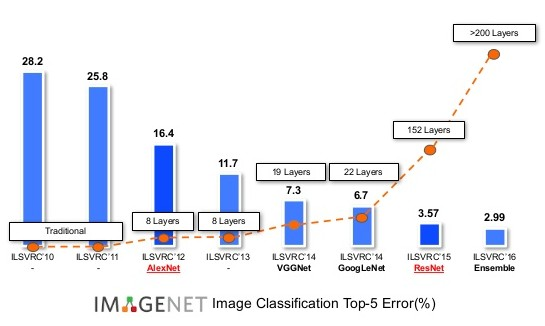
\includegraphics[width=0.8\textwidth]{img/compara_redes_ilsvrc.png}
\end{figure}


Apesar do foco inicial de DL ter sido concentrado no desenvolvimento de técnicas de aprendizado não-supervisionado e na habilidade de modelos profundos de boa generalização a partir de conjuntos de dados pequenos, o cenário atual das pesquisas nesta área consideram o uso de técnicas de aprendizado supervisionado bem mais antigas, visando o endereçamento de conjuntos de dados massivos e categorizados. \todo{Citar aqui} Nesta perspectiva encontram-se as redes neurais convolucionais com múltiplas camadas, que impulsionaram os avanços recentes na área de Visão Computacional \todo{idem, citar.}. Considerando esta importância, a seção a seguir compreenderá a explanação destes modelos, com especial para arquiteturas canônicas de maior destaque nos últimos anos.

\subsubsection{Redes Neurais Convolucionais} \label{subsubsec:rnc}

\emph{Redes Neurais Convolucionais} (CNN, do inglês \emph{Convolutional Neural Networks}) são uma classe de redes neurais \emph{feedforward} com topologia bem definida e estruturada em uma grade, com o uso de operações de convolução em pelo menos uma de suas camadas \cite{goodfellow2016deep}. Aplicadas em tarefas de classificação, regressão, localização, detecção e outras, este tipo de modelo se destaca no reconhecimento de padrões em dados de alta dimensionalidade, a exemplo de séries temporais, imagens e vídeos \cite{Khan:Livro}.

A operação de convolução possui um papel central nas CNNs. Esta operação descreve a média ponderada de uma determinada função $x_1(t)$ sob um intervalo fixo de uma variável, enquanto os pesos da média ponderada considerada pertencem à função $x_2(t)$ amostrados em intervalos $a$ \cite{bracewell1986fourier}. Assim, a convolução $s(t)$ de duas funções $x_1(t)$ e $x_2(t)$ é uma função $s: \mathds{Z} \rightarrow \mathds{R}$, denotada $s(t) = x_1(t) * x_2(t)$, e definida conforme Equação \ref{eq:int_convolucao} \cite{lathi2006sinais}:

\begin{equation}\label{eq:int_convolucao}
s(t) = x_1(t) * x_2(t) = \int_{-\infty}^{\infty} x_1(a) x_2(t-a)da.
\end{equation}

No contexto de ML, a função $x_1(t)$ é chamada de \emph{input}, a função $x_2(t)$ é o \emph{kernel}, e a saída $s(t)$ consiste no \emph{feature map}, ou mapa de características. No contexto prático, o \emph{input} normalmente é um vetor multidimensional de dados e o \emph{kernel} é um vetor multidimensional de pesos que devem ser ajustados para aprendizado das CNN. Considerando, por exemplo, uma imagem $I$ de dimensões $(m,n)$ como \emph{input} e a aplicação de um \emph{kernel} $K$, a versão discreta da convolução, passível de implementação computacional e equivalente à Eq. \ref{eq:int_convolucao}, é mostrada na Eq. \ref{eq:conv_img}:

\begin{equation}
 S(i,j) = I(i,j)*K(i,j) = \sum_{m}\sum_{n}I(m,n)K(i-m,j-n),\label{eq:conv_img}
\end{equation}
em que $S$ é o \emph{feature map} resultante e $(i,j)$ é a posição correspondente nesse mapa. Para otimizar os aspectos de implementação, os valores resultantes da operação de convolução são armazenados apenas nas posições $(i,j)$ explicitamente declaradas \cite{goodfellow2016deep}.

Os \emph{feature maps}, resultantes das operações de convolução, compreendem a noção de filtros, responsáveis por capturarem características relativas à entrada, tais como contornos, linhas, texturas, etc. Quando combinados de maneira sequencial, como proposto pelas CNNs, as características capturadas pelas camadas convolucionais vão se tornando mais complexas à medida que se aumenta a profundidade da rede. Assim, um primeiro \emph{feature map} de uma camada convolucional captura um simples contorno, enquanto um \emph{feature map} em uma camada mais profunda da rede pode capturar uma forma, um rosto ou até um objeto inteiro \cite{Buduma:Livro}. Esta noção é ilustrada na Figura \ref{fig:convolutions}.

\begin{figure}[!h]
	\centering
	\caption{Papel das camadas convolucionais e \emph{feature maps} nas CNNs. Fonte: \cite{Khan:Livro}.}
	\label{fig:convolutions}
	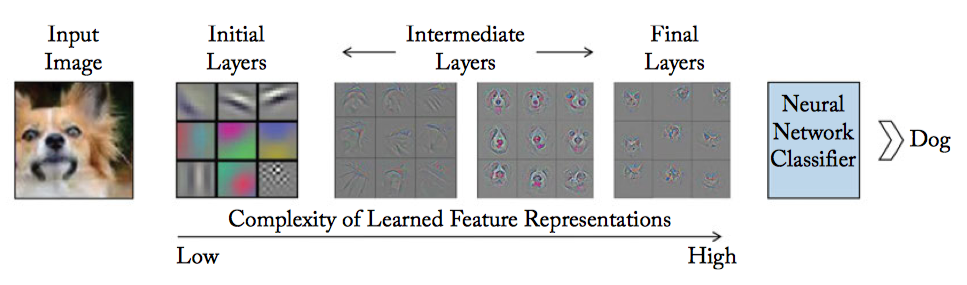
\includegraphics[width=0.8\textwidth]{./img/fundamenta/convolutions}
\end{figure}

As camadas convolucionais, que contém os \emph{feature maps} e os pesos da rede, normalmente são seguidas por funções de ativação não-linear.


A nonlinear function can also be understood as a switching or a selection mechanism, which decides whether a neuron will fire or not given all of its inputs. The activation functions that are commonly used in deep networks are differentiable to enable error back propagation

A toda camada convolucional em uma CNN, segue-se uma ativação não-linear, finalizando em uma operação de \emph{pooling}, como mostra a Figura \ref{fig:cnn_camada}. A seguir, serão explanadas cada uma destas etapas.


\begin{figure}
	\centering
	\caption{Componentes de uma camada de uma rede neural convolucional \cite{goodfellow2016deep}.}
	\label{fig:cnn_camada}
	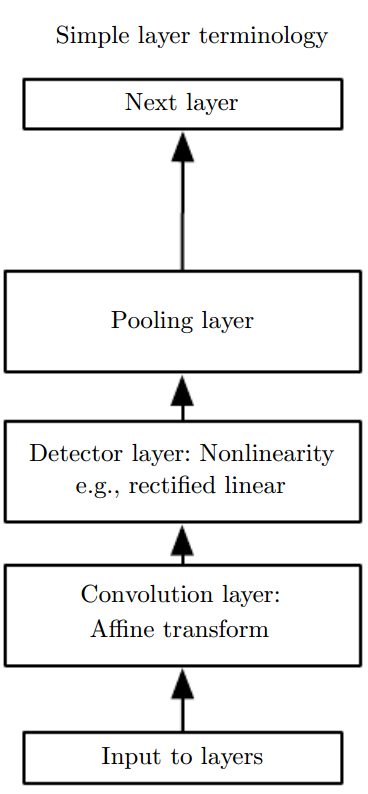
\includegraphics[height=0.3\textheight]{img/cnn_camada.png}
\end{figure}


\paragraph{Convolução}
\ \ \newline
A operação de convolução

Quando a operação de convolução é

A convolução é comutativa, ou seja, as Equações \ref{eq:conv_img_eq} e \ref{eq:conv_img} são equivalentes, salvo que no primeiro caso há a convolução da imagem pelo núcleo, enquanto no segundo há a convolução do núcleo pela imagem. Comumente, a Equação \ref{eq:conv_img} é a implementada em algoritmos de redes neurais convolucionais, haja visto que existem menor variação no intervalo de valores válidos de $m$ e $n$, o que diminui o custo computacional.

\begin{equation}\label{eq:conv_img_eq}
	S(i,j) = K(i,j)*I(i,j) = \sum_{m}\sum_{n}I(i-m,j-n)K(m,n)
\end{equation}

Logo após a operação de convolução, há a camada de ativação
\paragraph{Pooling}
\ \ \newline
Depois de realizar várias operações de convolução em paralelo para gerar um conjunto de ativações lineares e alimentá-las a funções de ativação não-lineares, como \emph{ReLU}, \emph{Softmax}, etc, na chamada etapa de detecção, chega-se à etapa de \emph{pooling}. Uma função de \emph{pooling} substitui a saída da rede em determinada localização por uma síntese estatística das saídas vizinhas. Por exemplo, a função \emph{max pooling} retorna o valor máximo em uma área retangular, enquanto a \emph{average pooling} retorna a média das saídas de um retângulo. %O objetivo destas funções é fazer com que


\subsubsection{Modelos Canônicos de Redes Neurais Convolucionais para Detecção de Objetos em Imagens} \label{subsubsec:modelos_canonicos}
